\documentclass[final,size=a3]{beamer}

% Description of files
%		beamerposter			-> package for making poster
%		beamerposterconfposter	-> template (modified by me)
%		images/					-> put all images here
%		sources.bib				-> bibliography
%		poster.tex				-> to make poster (this file)
% 		poster.pdf				-> poster output (send to SFU)

% References
\usepackage{apacite} 
\usepackage{lipsum}
\usepackage{scrextend}

\bibliographystyle{apacite}

% Case Competition poster style
\usepackage[scale=1.24]{beamerposter} 
\usetheme{confposter}

\setbeamertemplate{enumerate items}[default]

% Block titles
\setbeamercolor{block title}{fg=dblue,bg=white} 

% Body of blocks
\setbeamercolor{block body}{fg=black,bg=white} 

% Highlighted block titles
\setbeamercolor{block alerted title}{fg=white,bg=dblue!70}

% Body of highlighted blocks 
\setbeamercolor{block alerted body}{fg=black,bg=dblue!10} 

% sepwid is 0.024
\newlength{\sepwid}
\newlength{\onecolwid}
\newlength{\twocolwid}
\newlength{\threecolwid}

% Poster Dimensions:
%		48in x 36in
\setlength{\paperwidth}{48in} 
\setlength{\paperheight}{36in}
\setlength{\sepwid}{0.024\paperwidth} 

\setlength{\onecolwid}{0.22\paperwidth} 

% Set twocolwid to be (2*onecolwid)+sepwid = 0.464
\setlength{\twocolwid}{0.464\paperwidth} 

% (3*onecolwid)+2*sepwid = 0.708
\setlength{\threecolwid}{0.708\paperwidth}

% Set threecolwid to be (3*onecolwid)+2*sepwid = 0.708
\setlength{\threecolwid}{0.708\paperwidth} 
\setlength{\topmargin}{-0.5in} % Reduce the top margin size

% Required for including images
\usepackage{graphicx}  

% Top and bottom rules for tables
\usepackage{booktabs} 

% Poster title
\title{Case Study Competition \\ \vspace{8mm} \normalsize{Analysis of a Uken Games mobile app} \vspace{-5mm}} 

% Author(s)
\author{Nathan Esau, Steve Kane} 

% Institution(s) or Date of Competition
\institute{September 2015} 

\begin{document}

%\logo{sfu_logo}

% White space under blocks
\addtobeamertemplate{block end}{}{\vspace*{2ex}} 

% White space under highlighted (alert) blocks
\addtobeamertemplate{block alerted end}{}{\vspace*{2ex}} 

% White space under figures
\setlength{\belowcaptionskip}{0ex} 

% White space under equations
\setlength\belowdisplayshortskip{2ex} 

% The whole poster is enclosed in one beamer frame
\begin{frame}[t] 

% C1 -> W1
% C2 -> W3
%	C2A
%		C2A1 -> W0.48
%		C2A2 -> W0.52
% 	C2B 
%		C2B1 -> W0.33
% 		C2B2 -> W0.33
%		C2B3 -> W0.33

% C
\begin{columns}[t]

% C1 separator
\begin{column}{\sepwid}
\end{column} % C1 separator END

% C1 
\begin{column}{\onecolwid} 

% Objectives 
\begin{alertblock}{Objectives}
\normalsize
\begin{addmargin}[0.5em]{0em}
\begin{enumerate}[1.]
\item \ Come up with a good way to visualize the data that helps to provide explanatory insights
\item \ Use the demographic and event features to predict revenue, engagement and player retention
\item \ Suggest control-treatment experiments for follow up analysis
\end{enumerate}
\end{addmargin}

\end{alertblock}

\begin{block}{Introduction}

\begin{tabular}{l p{13cm}}
\textbf{Size training set: } & 250,000 players \\
\textbf{Size validation set: } & 50,000 players \\ 
\textbf{Types of variables: } & Country, gender, dates of in-game events, in-game purchases, prizes won; about 40 variables
\end{tabular}

\vspace{10mm}
\textbf{Revenue} measures the amount of money spent, while \textbf{Engagement} measures the amount of time spent in game. \textbf{Retention} indicates whether a player plays the game 30 days after installation.

\begin{itemize}
\item \texttt{Revenue} and \texttt{engagement} are \textbf{heavily} skewed
\item \texttt{97.8\%} of players don't spend money
\item Given that players pay, the average is \texttt{\$3.33} with only \texttt{5\%} paying more than \texttt{\$13.20}
\item The average time spent playing is \texttt{32.75}, but the median time spent playing is only \texttt{7}.
\item \texttt{Retention}: \texttt{9\%} of players returned 30 days later
\end{itemize}

\vspace{-5mm}
\begin{figure}
\caption{Important features for predicting revenue}
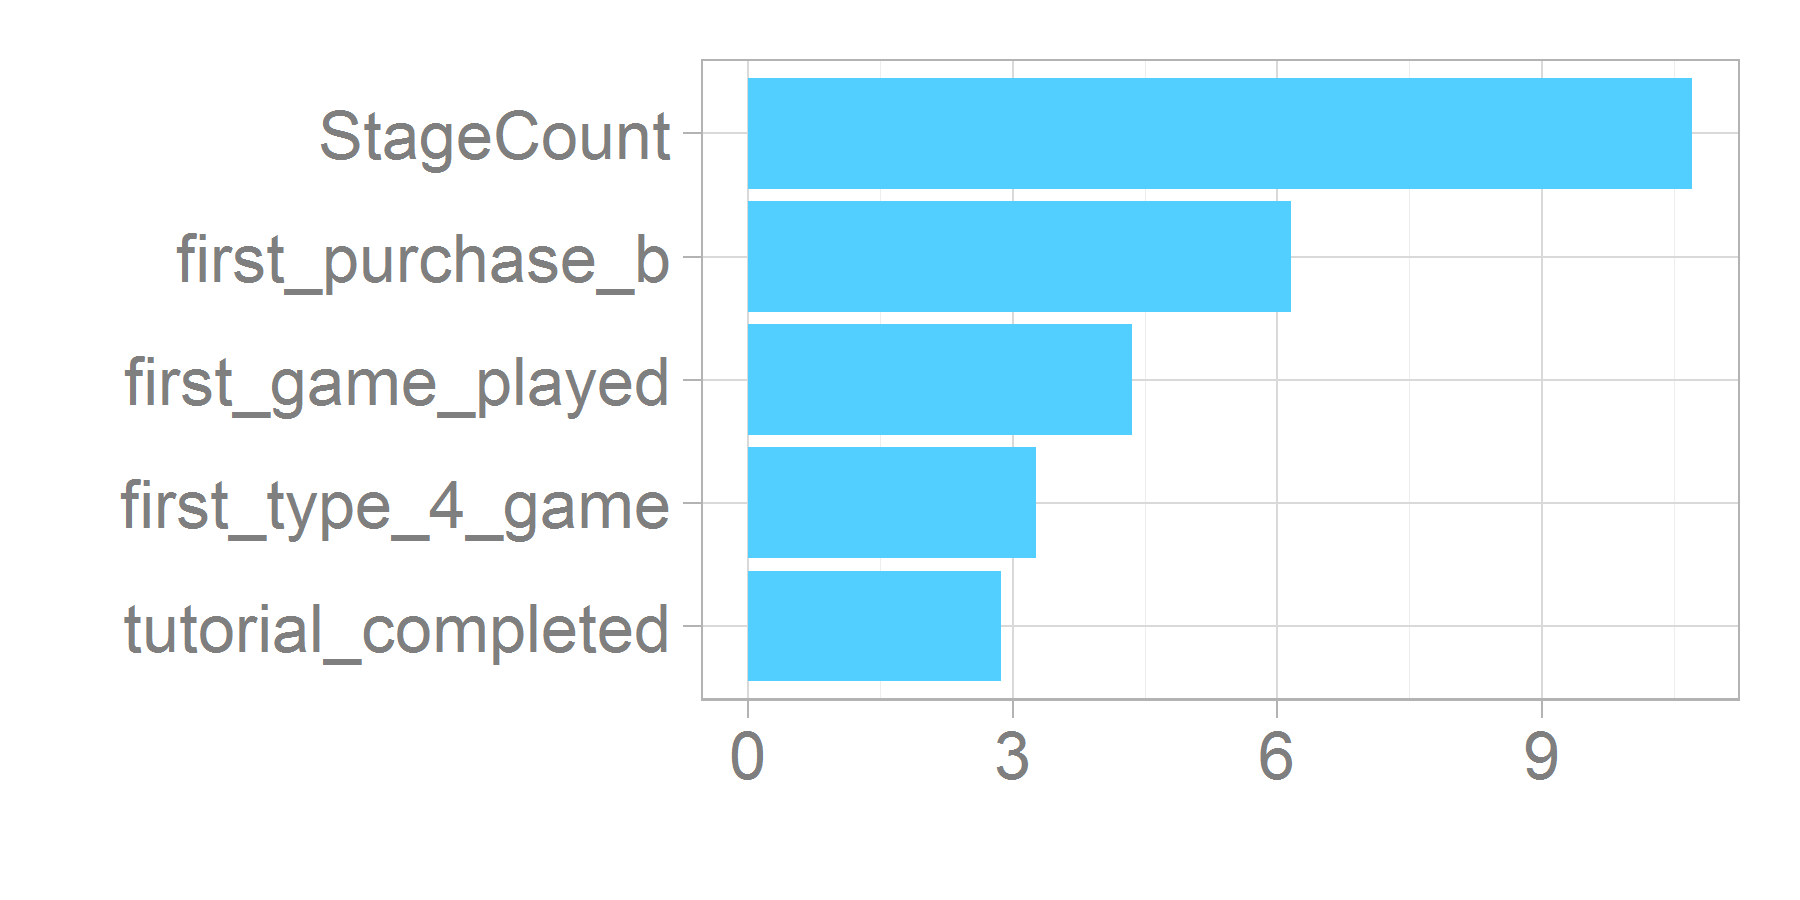
\includegraphics[width=0.9\linewidth]{images/Revenue_Feature_Importance}
\vspace{-5mm}
\end{figure}

\vspace{-15mm}
\begin{figure}
\caption{Important features for predicting engagement}
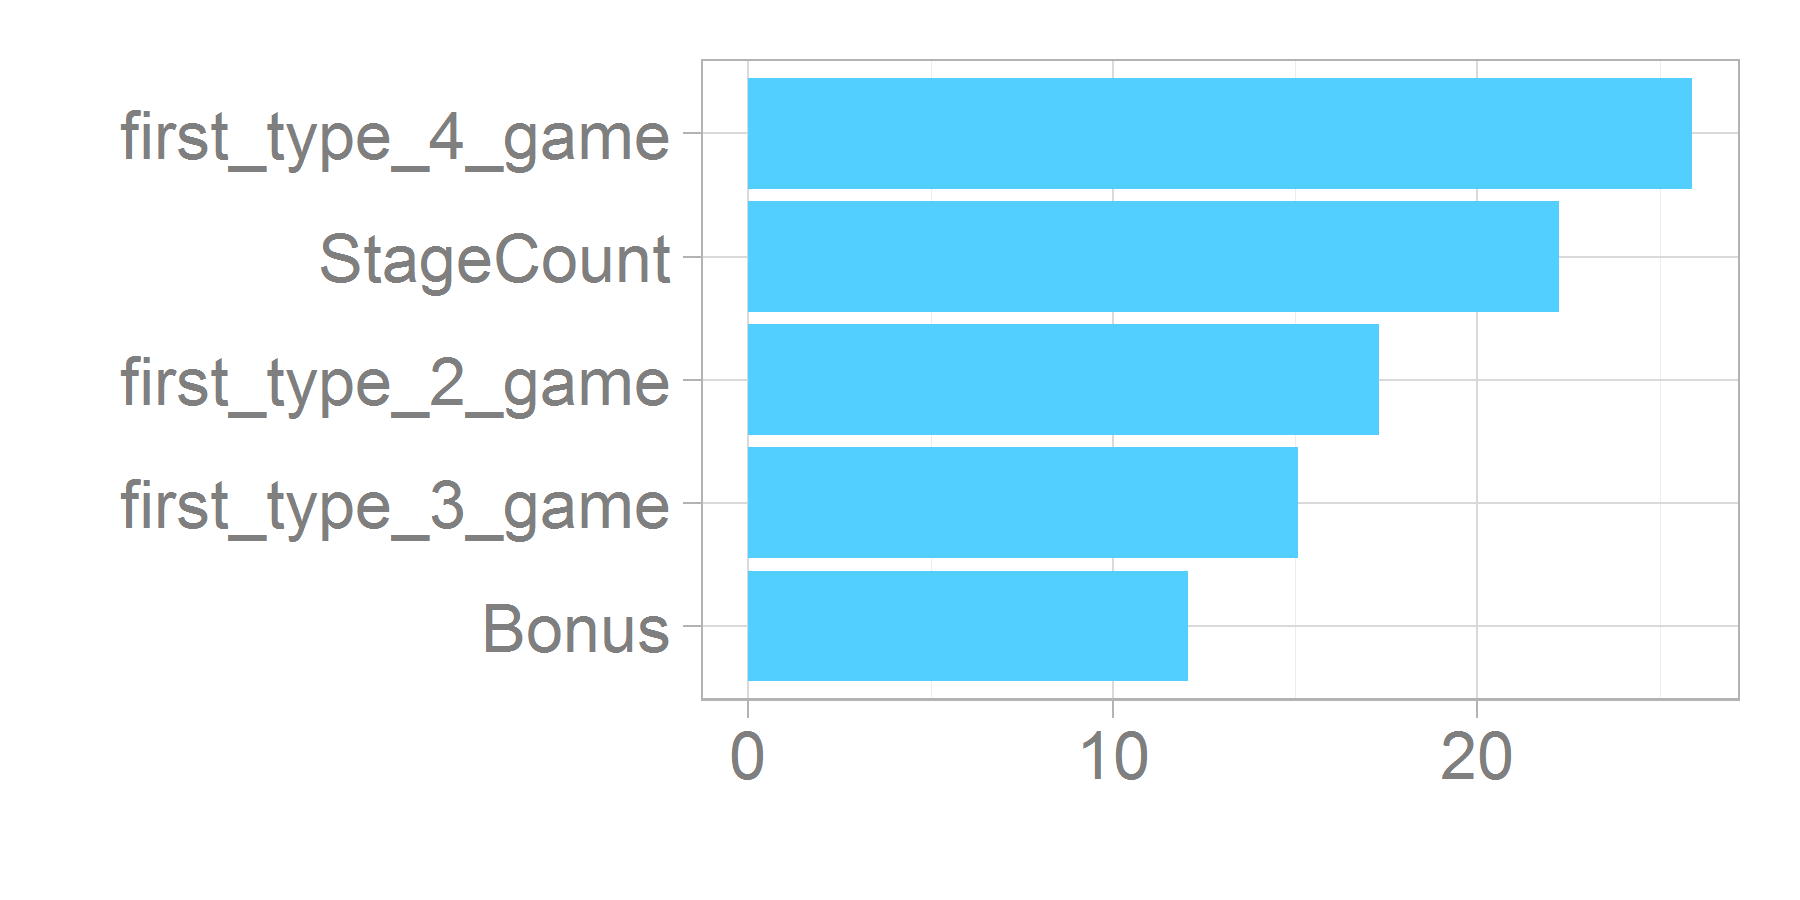
\includegraphics[width=0.9\linewidth]{images/Engagement_Feature_Importance}
\vspace{-5mm}
\end{figure}

\begin{itemize}
\item 
\end{itemize}

More \texttt{stuff} after that to fill the column.

\end{block}

\end{column} % C1 END

% C2 separator
\begin{column}{\sepwid}
\end{column} % C2 separator END

% C2
\begin{column}{\threecolwid} % Begin a column which is two columns wide (column 2)

% C2A
\begin{columns}[t]

% C2A1
\begin{column}{0.48\threecolwid}

\vspace{-25mm}

\begin{figure}[h]
\caption{Stages played, \texttt{engagement}, \texttt{revenue}, player skill (\texttt{bonuses} completed)}
\vspace{0mm}
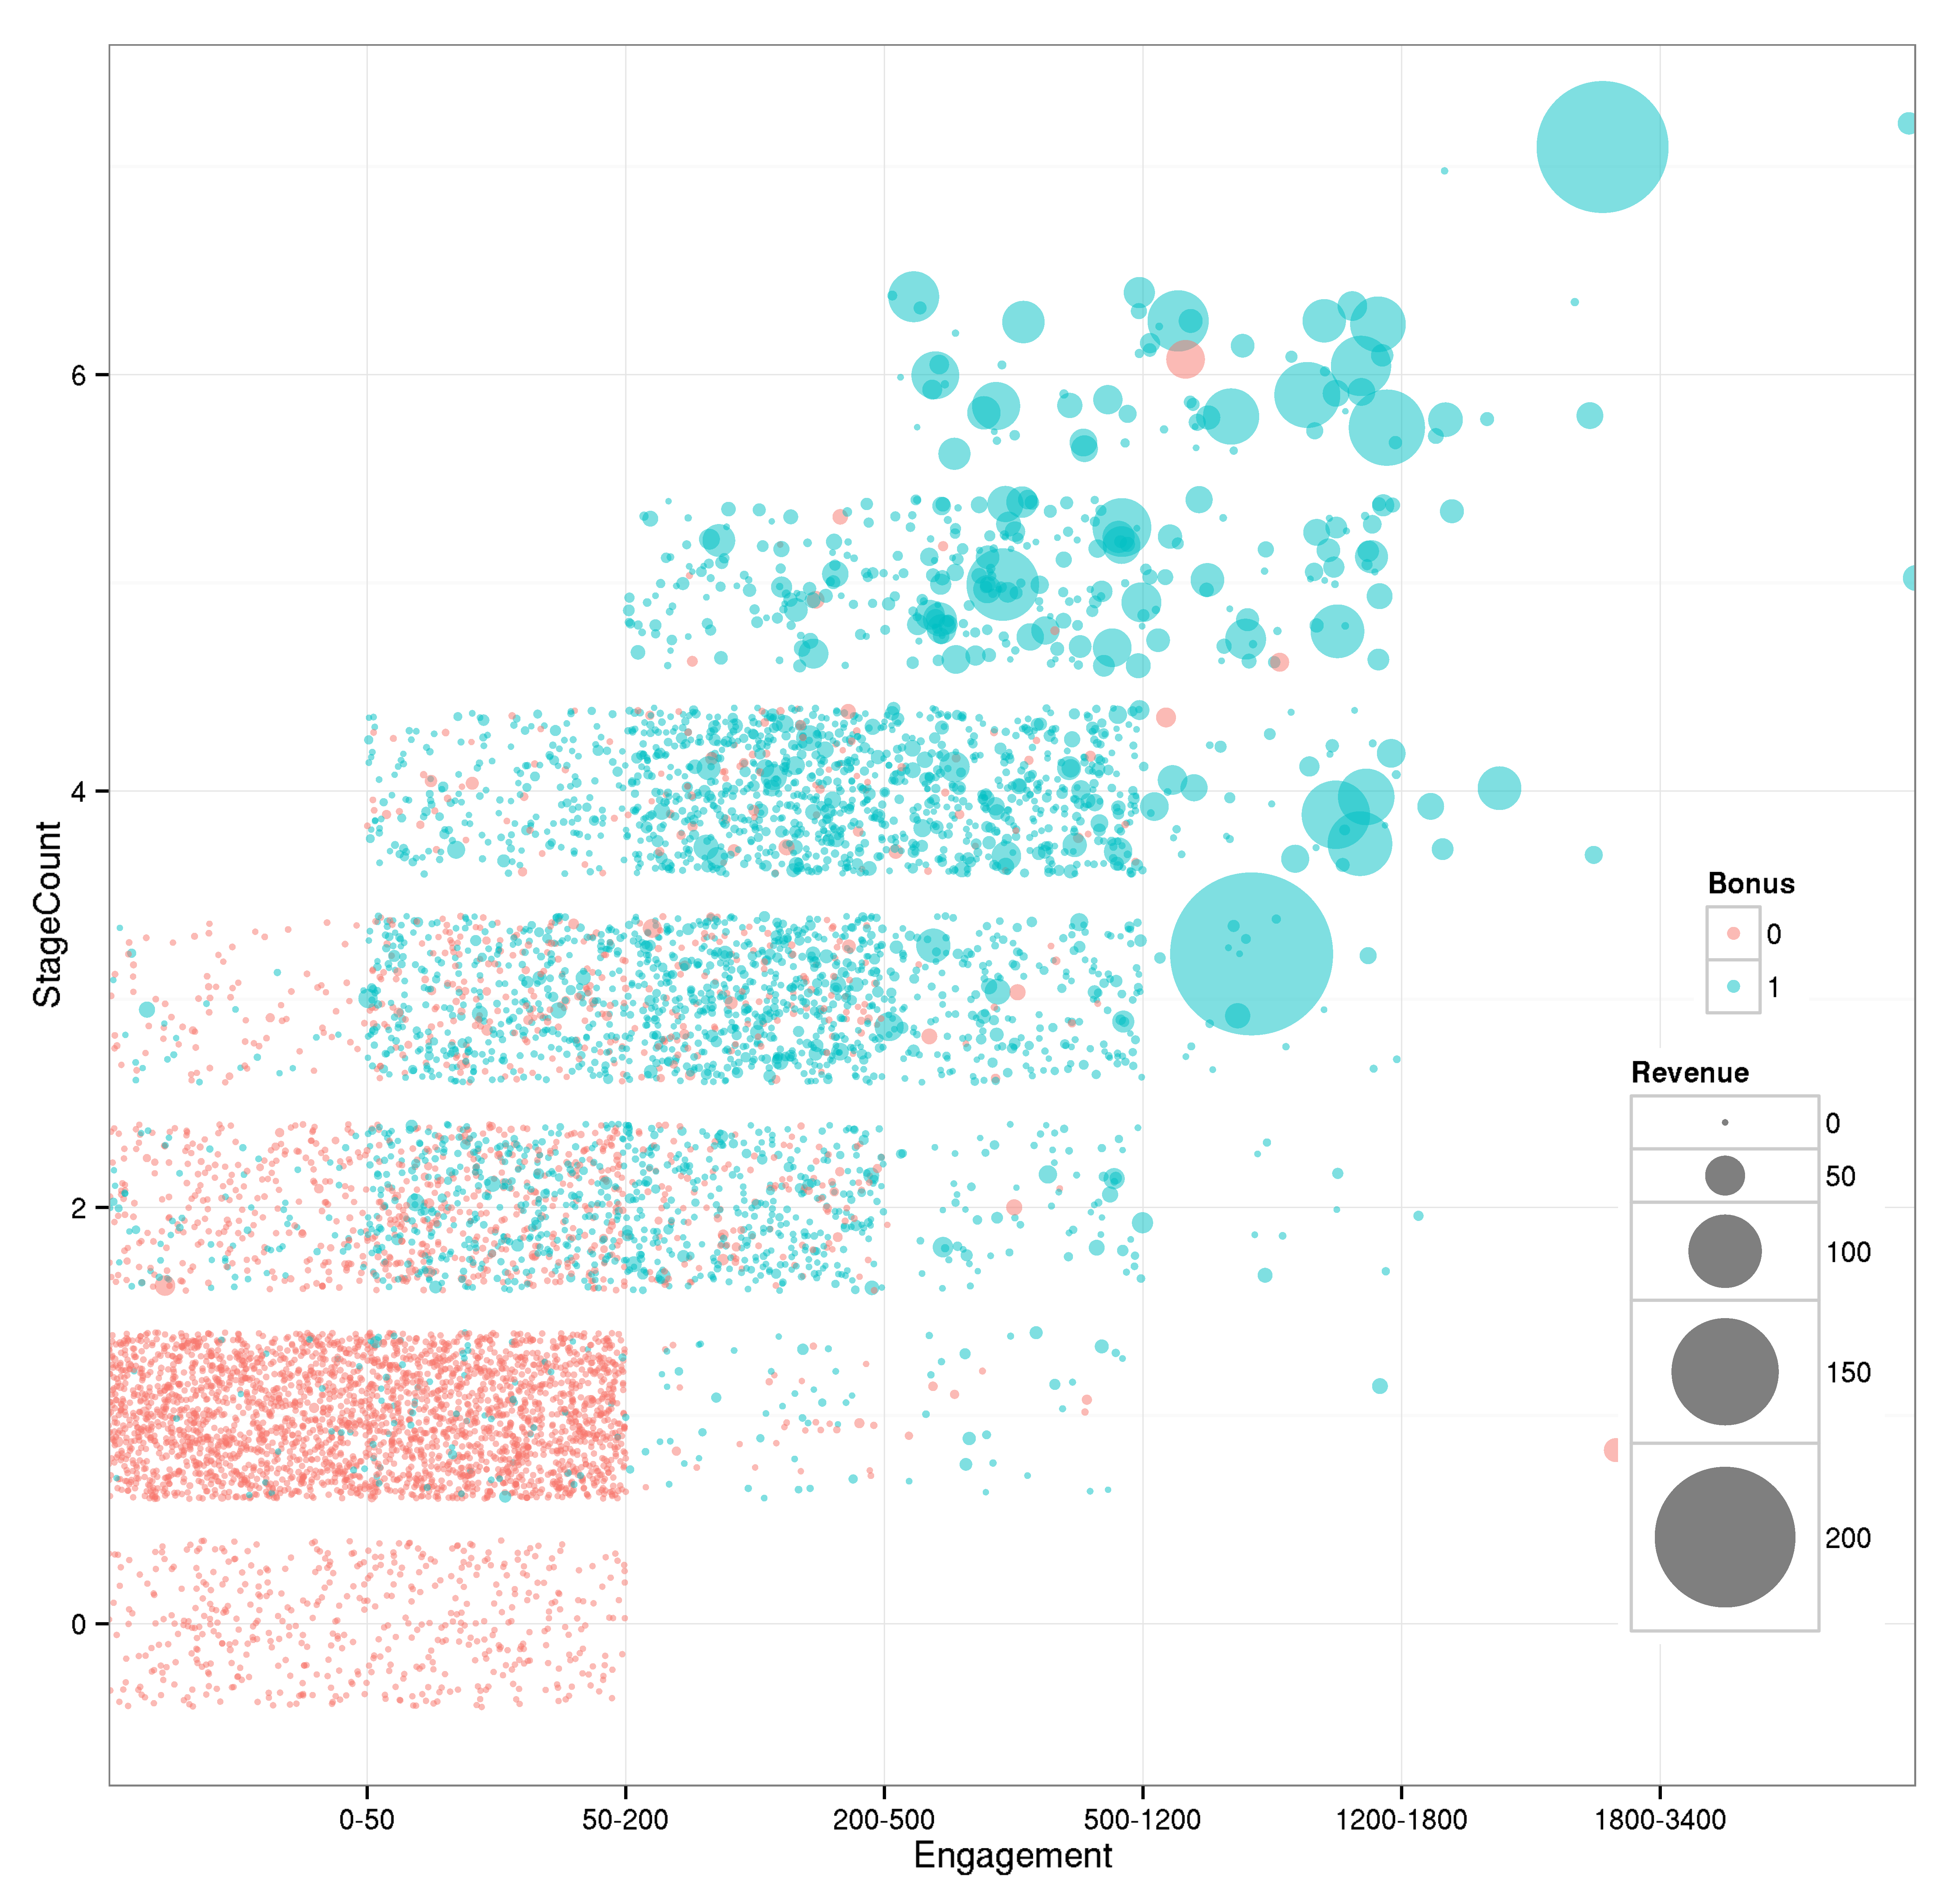
\includegraphics[scale=1.75]{images/bubsplot}
\end{figure}

\vspace{5mm}

\end{column} % C2A1 END

% C2A2
\begin{column}{0.52\threecolwid}

\vspace{-25mm}

\begin{figure}[h]
\caption{Heatmap for distribution of players from around the world}
\vspace{5mm}
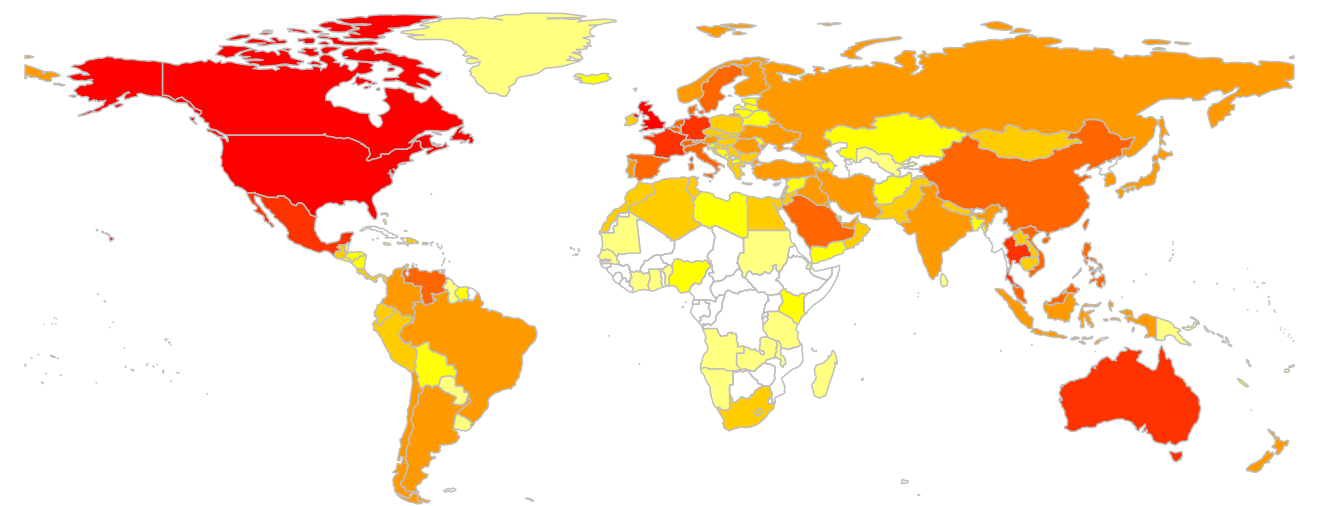
\includegraphics[scale=0.7]{images/world}
\end{figure}

\vspace{5mm}
\begin{block}{Predictions}

\begin{itemize}
\item We used the random forest model to predict \texttt{revenue} and \texttt{engagement} since this type of model works well with skewed data (Huang, 2005).
\item The gradient boosted model was used to predict \texttt{retention}. This model performed better than linear models we tried.
\end{itemize}

\vspace{-9mm}
\medskip
\def\arraystretch{1.4}
\begin{table}[h]
\caption{Comparison of prediction mean and training mean}
\vspace{3mm}
\begin{tabular}{|l| l l l|}
\hline 
& \ \texttt{Revenue} & \ \texttt{Engagement} & \ \texttt{Return Player} \\ \hline
\ Validation Mean \ & \ 3.31 $|$ Revenue > 0 & \ 33.33 & \ 6.5\% \\ \ Training Mean \ & \ 3.33 $|$ Revenue > 0 & \ 32.75 & \ 9.0\% \\ \hline
\end{tabular}
\vspace{5mm}
\end{table}

Note that the random forest model predicts 0 revenue for most of the new players, which is what we would expect.

\end{block}
\end{column} % C2A2 END

\end{columns} % C2A END

% C2B
\begin{columns}[t]

% C2B1
\begin{column}{0.333\threecolwid} % The first column within column 2 (column 2.1)

\begin{block}{Random Forest Model}

\vspace{-3mm}
\begin{figure}[h]
\caption{Simple decision tree}
\vspace{5mm}
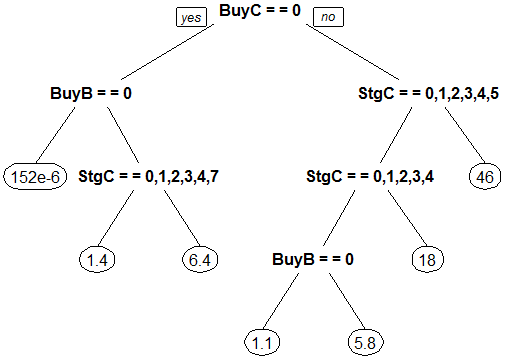
\includegraphics[scale=1.3]{images/SimpleTree}
\end{figure}

\vspace{-7mm}
\begin{figure}[ht]
\caption{A random forest}
\vspace{5mm}
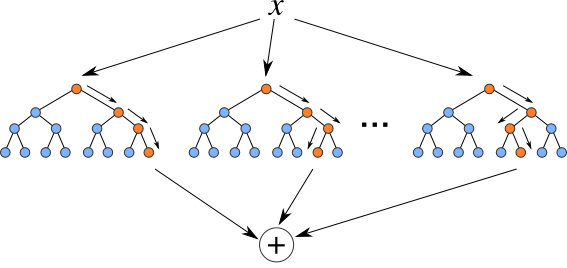
\includegraphics[scale=1.3]{images/randomForestGraph}
\end{figure}

\vspace{-3mm}
We create an \texttt{ensemble} of many unstable models to form a stable model.

\end{block}

\end{column} % C2B1 END

% C2B2
\begin{column}{0.33\threecolwid}

\begin{block}{Gradient Boosted Model}

\begin{figure}[h]
\caption{Error-complexity tradeoff}
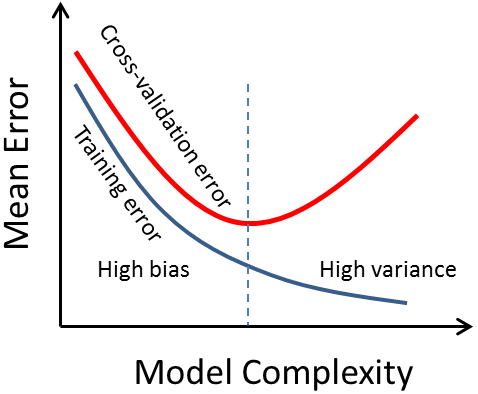
\includegraphics[scale=1.4]{images/error_complexity}
\end{figure}

%First, we determined the coefficients of a logistic regression model,
%
%\begin{equation*}
%\log \left( \frac{p}{1 - p} \right) = \beta_0 + \beta_1 X + \beta_2 X + \dots 
%\end{equation*}

%However, note that $F$ is modified by adding a function like so

We update our model, $F(x) = 0.5 \log \left(\frac{1 + \bar{y}}{1 - \bar{y}}\right)$ \\ by continually adding a new basis function to \\ minimize the loss function,

\vspace{-12mm}
\begin{equation*}
l(y_i, \hat{y}_i) = y_i \ln(1 + e^{-\hat{y}_i}) + (1 - y_i)\ln(1 + e^{\hat{y}_i})
\end{equation*}

\vspace{-2mm}
The gradient boosted model uses a \texttt{greedy} algorithm.

\end{block}

\end{column} % C2B2 END

\begin{column}{0.33\threecolwid}

\begin{block}{Conclusions}

\textbf{A/B tests to improve key metrics}
%
\begin{itemize}
\item Figure 3 shows that completing bonus objectives is likely to increase revenue. We expect that \textit{creating additional stages} or \textit{adjusting the difficulty} of the bonus objective could increase revenue.
\item It would be interesting to analyze the impact of providing unlockable features when a player the game connects to Facebook or another device.
\end{itemize}

\textbf{Relationship of key metrics}
%
\begin{itemize}
\item Stage Count is highly significant to both \texttt{engagement} and \texttt{revenue}
\item The types of games a player tries out is highly significant to \texttt{engagement}
\item The type of purchase a player made is very significant to \texttt{revenue}
\end{itemize}

\end{block}

\end{column}

\end{columns} % C2B END

\begin{columns} % C2C

\begin{column}{0.35\threecolwid}

% Random forest column

\end{column}

\begin{column}{0.65\threecolwid}

\vspace{-85mm}
\begin{alertblock}{References}

%\nocite{*}
%\bibliography{sources}
\small
\textbf{Analysis} was done using \texttt{R}. \url{http://www.R-project.org}. The \texttt{ggplot2}, \texttt{randomForest}, \texttt{data.table}, \texttt{xgboost}, \texttt{readr}, \texttt{qdapTools}, and \texttt{Matrix} packages were used. For the \textbf{models} see \textit{Methods to Extract Rare Events} by Weihua Huang. 2005.
% Paste the rest of the references

\end{alertblock}

\end{column} % C2C END

\end{columns}

\end{column} % C2 END

\end{columns} % C END

\end{frame} % End of the enclosing frame

\end{document}
